\documentclass{ximera}


\title{Continuity Activity Solution Guide}
\author{MATH 425: Calculus I}

\begin{document}
\begin{abstract}
     Working with the peers in your group, solve the following problems. Make sure to show and justify all your work. Make sure everyone in the group understands the solution and participates. Be prepared to report your answers to the whole class. 
\end{abstract}
\maketitle

\begin{exercise}
     Decide if each of the five given statements is true or false.  If the statement is false, provide a counterexample: sketch a graph of a function showing that the statement is false.  Then use another representation: a table, a symbolic equation, and/or words to explain why the graph you sketched disproves the statement. 
    \begin{enumerate}
        \item If $\lim_{x\rightarrow c}f(x)=f(c)$, then $f$ is continuous at $x=c$.  \\
        We think this statement is \textcolor{blue}{true}\\
        Justification (explain with words, a table, an equation or graph, OR provide a counterexample, if applicable):\\
        \textcolor{blue}{ This is the definition of a continuous function.  }
        \item If $f$ is not continuous at $x=c$, then $f(c)\neq \lim_{x\rightarrow c}f(x)$.\\
        We think this statement is \textcolor{blue}{true}\\
        Justification (explain with words, a table, an equation or graph, OR provide a counterexample, if applicable):\\
        \textcolor{blue}{Assuming that the function is not continous at $x=c$ means that either 
          \begin{enumerate}
            \item $f(c)$ is not defined 
            \item $\lim_{x\rightarrow c} f(x)$ DNE OR
            \item $\lim_{x\rightarrow c} f(x)\neq f(c)$ (but both are defined). 
          \end{enumerate}
          In all three cases, we know that $f(c)\neq \lim_{x\rightarrow c}f(x)$ (things that are not defined cannot be equal).}
        \item If $f$ is not continuous at $x=c$, then $f(c)$ is undefined.\\
        We think this statement is \textcolor{blue}{false}\\
        Justification (explain with words, a table, an equation or graph, OR provide a counterexample, if applicable):\\
        \textcolor{blue}{Counterexample (any function with a jump or removable continuity with a point defined for $f(c)$ will work):\\
        \[f(x)=\begin{cases}
        x+1 & x>1\\
        x & x\leq 1
        \end{cases}\]
        $f(1)=1$, which is defined, but the function jumps at $x=1$.}
        \item If $f$ is not continuous at $x=c$, then $\lim_{x\rightarrow c}f(x)$ does not exist.\\
        We think this statement is \textcolor{blue}{false}\\
        Justification (explain with words, a table, an equation or graph, OR provide a counterexample, if applicable):\\
        \textcolor{blue}{ Counterexample (any function with a removable discontinuity will do):
        \[f(x)=\frac{x}{x(x-1)}\]
        $f(0)$ is undefined because of division by 0, so $f(x)$ is not continuous at $x=0$, but 
        \[\lim_{x\rightarrow 0}\frac{x}{x(x-1)}=\lim_{x\rightarrow 0}\frac{1}{x-1}=\frac{1}{-1}=-1\] exists.}
        \item If $f$ is not continuous at $x=c$, then either $f(c)$ is undefined or $\lim_{x\rightarrow c}f(x)$ does not exist.\\
        We think this statement is \textcolor{blue}{false}\\
        Justification (explain with words, a table, an equation or graph, OR provide a counterexample, if applicable):
        \textcolor{blue}{Couterexample: (Any function with a removable discontinuity with an additional defined point for the discontinuity would work.)
        \[f(x)=
        \begin{cases}
         x+1 &  x\neq 2\\
         -2 & x=2
        \end{cases}\]
        We have that $f$ is not continuous at $x=2$, but $f(2)=-2$ and $\lim_{x\rightarrow 2}x+1=3$, so both are defined.}
        

        \item Which statements in part (a) through (e) match the following graphs:
        
      
        \begin{image}
        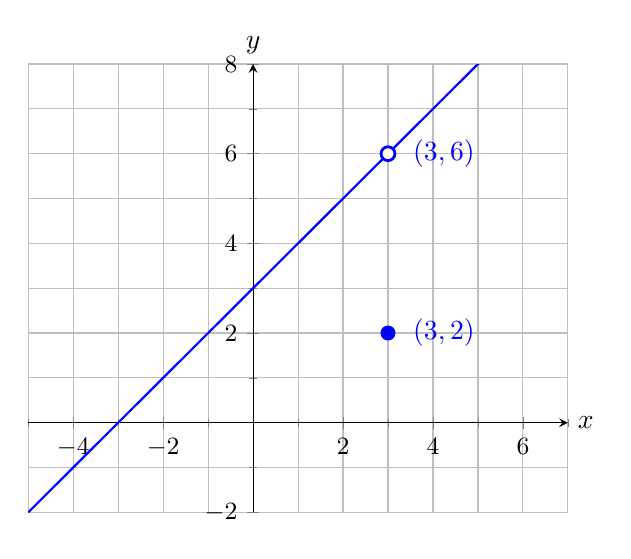
\begin{tikzpicture}
  \begin{axis}[
    axis lines=middle,
    xlabel={$x$},
    ylabel={$y$},
    xmin=-5, xmax=7,
    ymin=-2, ymax=8,
    grid=both,
    minor tick num=1,
    enlargelimits=false,
    ticklabel style={font=\small},
    every axis x label/.style={at={(current axis.right of origin)}, anchor=west},
    every axis y label/.style={at={(current axis.above origin)}, anchor=south},
  ]

    % y = x + 3 for all x (we’ll mark the hole at x=3 explicitly)
    \addplot[
      domain=-5:7,
      samples=200,
      thick,
      blue
    ] {x + 3};

   % White-filled dot
\addplot[
  only marks,
  mark=*,
  mark size=2.5pt,
  draw=none,
  fill=white
] coordinates {(3,6)};

% Blue ring on top
\addplot[
  only marks,
  mark=o,
  mark size=2.5pt,
  line width=1pt,
  draw=blue
] coordinates {(3,6)};
   

    % Filled dot at (3,2) for the defined value y=2 when x=3
    \addplot[
      only marks,
      mark=*,
      mark size=2.5pt,
      blue
    ] coordinates {(3,2)};

    % Optional: labels near the special points
    \node[anchor=west, blue] at (axis cs:3,6) {$\;\;(3,6)$};
    \node[anchor=west, blue]  at (axis cs:3,2) {$\;\;(3,2)$};

  \end{axis}
  
\end{tikzpicture}

\end{image}
    Graph A\\
      \xmalt{Graph of the function $y=x+3$ with a hole at $(3,6)$ and a point at $(3,2)$.}

\begin{image}
        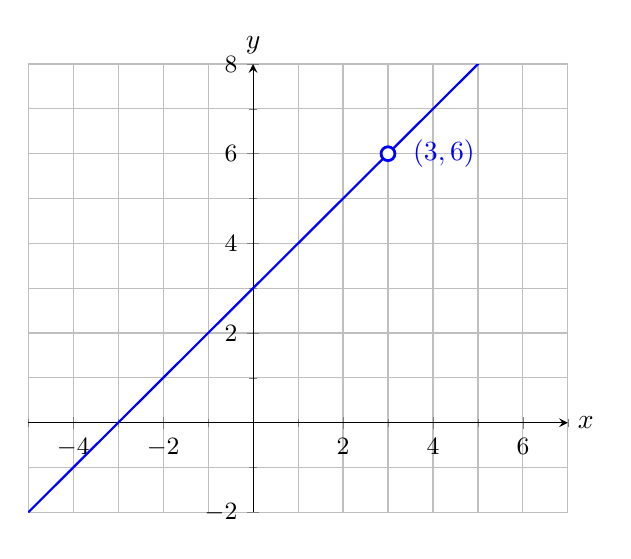
\begin{tikzpicture}
  \begin{axis}[
    axis lines=middle,
    xlabel={$x$},
    ylabel={$y$},
    xmin=-5, xmax=7,
    ymin=-2, ymax=8,
    grid=both,
    minor tick num=1,
    enlargelimits=false,
    ticklabel style={font=\small},
    every axis x label/.style={at={(current axis.right of origin)}, anchor=west},
    every axis y label/.style={at={(current axis.above origin)}, anchor=south},
  ]

    % y = x + 3 for all x (we’ll mark the hole at x=3 explicitly)
    \addplot[
      domain=-5:7,
      samples=200,
      thick,
      blue
    ] {x + 3};

    % White-filled dot
\addplot[
  only marks,
  mark=*,
  mark size=2.5pt,
  draw=none,
  fill=white
] coordinates {(3,6)};

% Blue ring on top
\addplot[
  only marks,
  mark=o,
  mark size=2.5pt,
  line width=1pt,
  draw=blue
] coordinates {(3,6)};
   

    % Optional: labels near the special points
    \node[anchor=west, blue] at (axis cs:3,6) {$\;\;(3,6)$};
    %\node[anchor=west, blue]  at (axis cs:3,2) {$\;\;(3,2)$};

  \end{axis}
 
\end{tikzpicture}

        \end{image}
        Graph B\\
        \xmalt{Graph of the function $y=x+3$ with a hole at the point $(3,6)$.}

        We think graph A matches with ... \textcolor{blue}{statement e}\\
        We think graph B matches with ... \textcolor{blue}{statement d}\\
        (Question modified from Straumanis et al., \textit{Calculus I: A Guided Inquiry}, 2014.)
    \end{enumerate}
\end{exercise}

\begin{exercise}
    Give an example of a single function $f(x)$ such that satisfies the following four characteristics:\\
    \begin{enumerate} 
        \item $f(x)$ is continuous everywhere except at $x=-2, 3$ and $4$
        \item $f(3)=5$
        \item $\lim_{x\rightarrow 2^-}f(x)=1$
        \item $\lim_{x\rightarrow 4}f(x)=6$
    \end{enumerate}


    (Hint: A symbolic equation is not the only way to represent a function.  A sketch of a graph may be an easier representation to use here.)\\
    
    \textcolor{blue}{Many graphs are possible, but here is one example: }
    \begin{image}
    \includegraphics{continuity2A.png}
    \end{image}
    
    (Questions modified from Boelkins, et al., \textit{Active Calculus}, 1st ed.)
\end{exercise}

\begin{exercise}
  Analyze the continuity of the function:\\

\[ f(x) = 
  \begin{cases} 
     x^2+1 & \text{if } x < -3 \\ 
     -2x+4 & \text{if } -3 \leq x < 2 \\
     \dfrac{1}{2}x^2 & \text{if } x \geq 2 
  \end{cases}  \]

(When analyzing the continuity of a function, you should identify any places where the function is discontinuous, the type of discontinuity, and give a (brief) explanation or show work for anywhere the function is continuous.)\\
\textcolor{blue}{When $x<-3$, the function is given by $x^2+1$, which is a polynomial and thus continuous.\\
At $x=-3$,\\
$\lim_{x\rightarrow -3^-}f(x)=\lim_{x\rightarrow -3^-}x^2+1=(-3)^2+1=10$\\
$\lim_{x\rightarrow -3^+}f(x)=\lim_{x\rightarrow -3^+} -2x+4=-2(-3)+4=10$\\
So $\lim_{x\rightarrow -3}f(x)=10=f(-3)$.  The function is continuous at $x=-3$.
When $-3< x<2$, the function is given by $-2x+4$, which is a polynomial, and thus continuous.\\
At $x=2$, \\
$\lim_{x\rightarrow 2^-}f(x)=\lim_{x\rightarrow 2^-}-2x+4=-2(2)+4=0$\\
$\lim_{x\rightarrow 2^+}f(x)=\lim_{x\rightarrow 2^+} \frac{1}{2}x^2=\frac12(2^2)=2$\\
So $\lim_{x\rightarrow 2}f(x)$ DNE, and the function has a jump discontinuity at $x=2$.  
When $x>2$, the function is given by $\frac12 x^2$, which is a polynomial and thus continuous.}

\end{exercise}


\end{document}